\noindent
\begin{minipage}[t]{0.26\textwidth}
    \vspace*{7.4cm}
    \raggedright\small
    Đồ thị của các hàm số $y$ và $y'$ trong Ví dụ~6 được thể hiện trong Hình~1. Chú ý rằng $y'$ nhận giá trị lớn khi $y$ tăng nhanh và $y' = 0$ khi $y$ có tiếp tuyến nằm ngang. Vì vậy kết quả của chúng ta có vẻ rất hợp lý.
    
    \vspace{0.35cm}
    \centering
    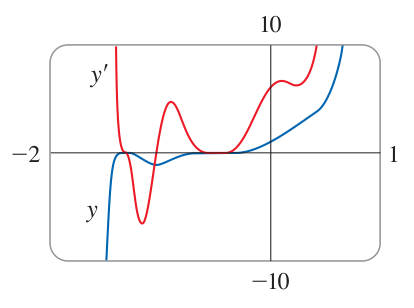
\includegraphics[width=\linewidth]{images/p0238_fig1.png}
    
    \vspace{0.2cm}
    \raggedright
    \textbf{\textsf{HÌNH 1}}
    
    \vspace{2.1cm}
    \raggedright\small
    Tổng quát hơn, Quy tắc chuỗi cho ta
    \begin{equation*}
        \frac{d}{dx}(e^u) = e^u \frac{du}{dx}
    \end{equation*}
\end{minipage}%
\hfill
\begin{minipage}[t]{0.71\textwidth}
    \textbf{\textsf{\color{stewartcyan}VÍ DỤ 5}}\quad Tìm đạo hàm của hàm số
    \begin{equation*}
        g(t) = \left( \frac{t - 2}{2t + 1} \right)^9
    \end{equation*}

    \textbf{\textsf{\color{stewartcyan}LỜI GIẢI}}\quad Kết hợp Quy tắc lũy thừa, Quy tắc chuỗi và Quy tắc thương, ta có
    \begin{align*}
        g'(t) &= 9 \left( \frac{t - 2}{2t + 1} \right)^8 \frac{d}{dt} \left( \frac{t - 2}{2t + 1} \right) \\[6pt]
        &= 9 \left( \frac{t - 2}{2t + 1} \right)^8 \frac{(2t + 1) \cdot 1 - 2(t - 2)}{(2t + 1)^2} = \frac{45(t - 2)^8}{(2t + 1)^{10}} \tag*{\color{stewartcyan}\blacksquare}
    \end{align*}

    \vspace{0.35cm}
    \textbf{\textsf{\color{stewartcyan}VÍ DỤ 6}}\quad Tính đạo hàm của $y = (2x + 1)^5 (x^3 - x + 1)^4$.

    \textbf{\textsf{\color{stewartcyan}LỜI GIẢI}}\quad Trong ví dụ này, chúng ta phải sử dụng Quy tắc tích trước khi dùng Quy tắc chuỗi:
    \begin{align*}
        \frac{dy}{dx} &= (2x + 1)^5 \frac{d}{dx}(x^3 - x + 1)^4 + (x^3 - x + 1)^4 \frac{d}{dx}(2x + 1)^5 \\[6pt]
        &= (2x + 1)^5 \cdot 4(x^3 - x + 1)^3 \frac{d}{dx}(x^3 - x + 1) \\
        &\qquad\qquad + (x^3 - x + 1)^4 \cdot 5(2x + 1)^4 \frac{d}{dx}(2x + 1) \\[6pt]
        &= 4(2x + 1)^5 (x^3 - x + 1)^3 (3x^2 - 1) + 5(x^3 - x + 1)^4 (2x + 1)^4 \cdot 2
    \end{align*}
    Nhận thấy rằng mỗi số hạng đều có nhân tử chung là $2(2x + 1)^4 (x^3 - x + 1)^3$, ta có thể đặt nhân tử chung này ra ngoài và viết câu trả lời dưới dạng
    \begin{equation*}
        \frac{dy}{dx} = 2(2x + 1)^4 (x^3 - x + 1)^3 (17x^3 + 6x^2 - 9x + 3) \tag*{\color{stewartcyan}\blacksquare}
    \end{equation*}

    \vspace{0.35cm}
    \textbf{\textsf{\color{stewartcyan}VÍ DỤ 7}}\quad Tính đạo hàm của $y = e^{\sin x}$.

    \textbf{\textsf{\color{stewartcyan}LỜI GIẢI}}\quad Ở đây hàm bên trong là $g(x) = \sin x$ và hàm bên ngoài là hàm mũ $f(x) = e^x$. Do đó, theo Quy tắc chuỗi,
    \begin{equation*}
        \frac{dy}{dx} = \frac{d}{dx}(e^{\sin x}) = e^{\sin x} \frac{d}{dx}(\sin x) = e^{\sin x} \cos x \tag*{\color{stewartcyan}\blacksquare}
    \end{equation*}

    \vspace{0.45cm}
    Lý do cho tên gọi “Quy tắc chuỗi” trở nên rõ ràng hơn khi ta thiết lập một chuỗi dài hơn bằng cách bổ sung thêm một mắt xích. Giả sử $y = f(u)$, $u = g(x)$ và $x = h(t)$, trong đó $f, g$ và $h$ đều là các hàm khả vi. Khi đó, để tính đạo hàm của $y$ theo biến $t$, ta sử dụng Quy tắc chuỗi hai lần:
    \begin{equation*}
        \frac{dy}{dt} = \frac{dy}{dx} \frac{dx}{dt} = \frac{dy}{du} \frac{du}{dx} \frac{dx}{dt}
    \end{equation*}
\end{minipage}

\vfill
\begin{center}
    \fontsize{6.5pt}{8pt}\selectfont \color{stewartgray}
    Copyright 2021 Cengage Learning. All Rights Reserved. May not be copied, scanned, or duplicated, in whole or in part. WCN 02-200-203\\
    Bản dịch tiếng Việt phục vụ mục đích học tập và nghiên cứu theo giáo trình chuẩn quốc tế.
\end{center}
